% !TEX root = ../main.tex
% !TEX program = xelatex
\section{问题重述}
\subsection{问题背景}
微网是一种将分布式发电、储能设备和用电负载进行统一协调的小型供电系统，能够提高本地能源的利用效率，并减少对外部电网的依赖。
如图\ref{fig:weiwang}所示，微网中的电力来自光伏发电和外部电网。
光伏发出的电可以优先满足小区负载；当光伏有剩余时，可以将多余电量存入储能设备；当光伏不足时，则可以由储能设备放电或从外部电网购电来补充。

外网电价较低时，微网可以提前购电并存入储能设备，在之后电价较高或供电不足时使用。
因此，微网每天都需要解决一个调度问题：\textbf{各时段应该购买多少电，储能设备何时充电、何时放电。}

买电过多会增加费用，买电过少又可能在实际运行中产生高价补购；
同时，储能设备还受到容量、充放电功率和充放电效率等条件的限制。
因此，需要结合供需预测、储能状态和电价，协调购电与充放电，在保证小区正常供电和储能安全运行的前提下，使总购电费用尽可能低。

\begin{figure}[!htbp]
    \centering
    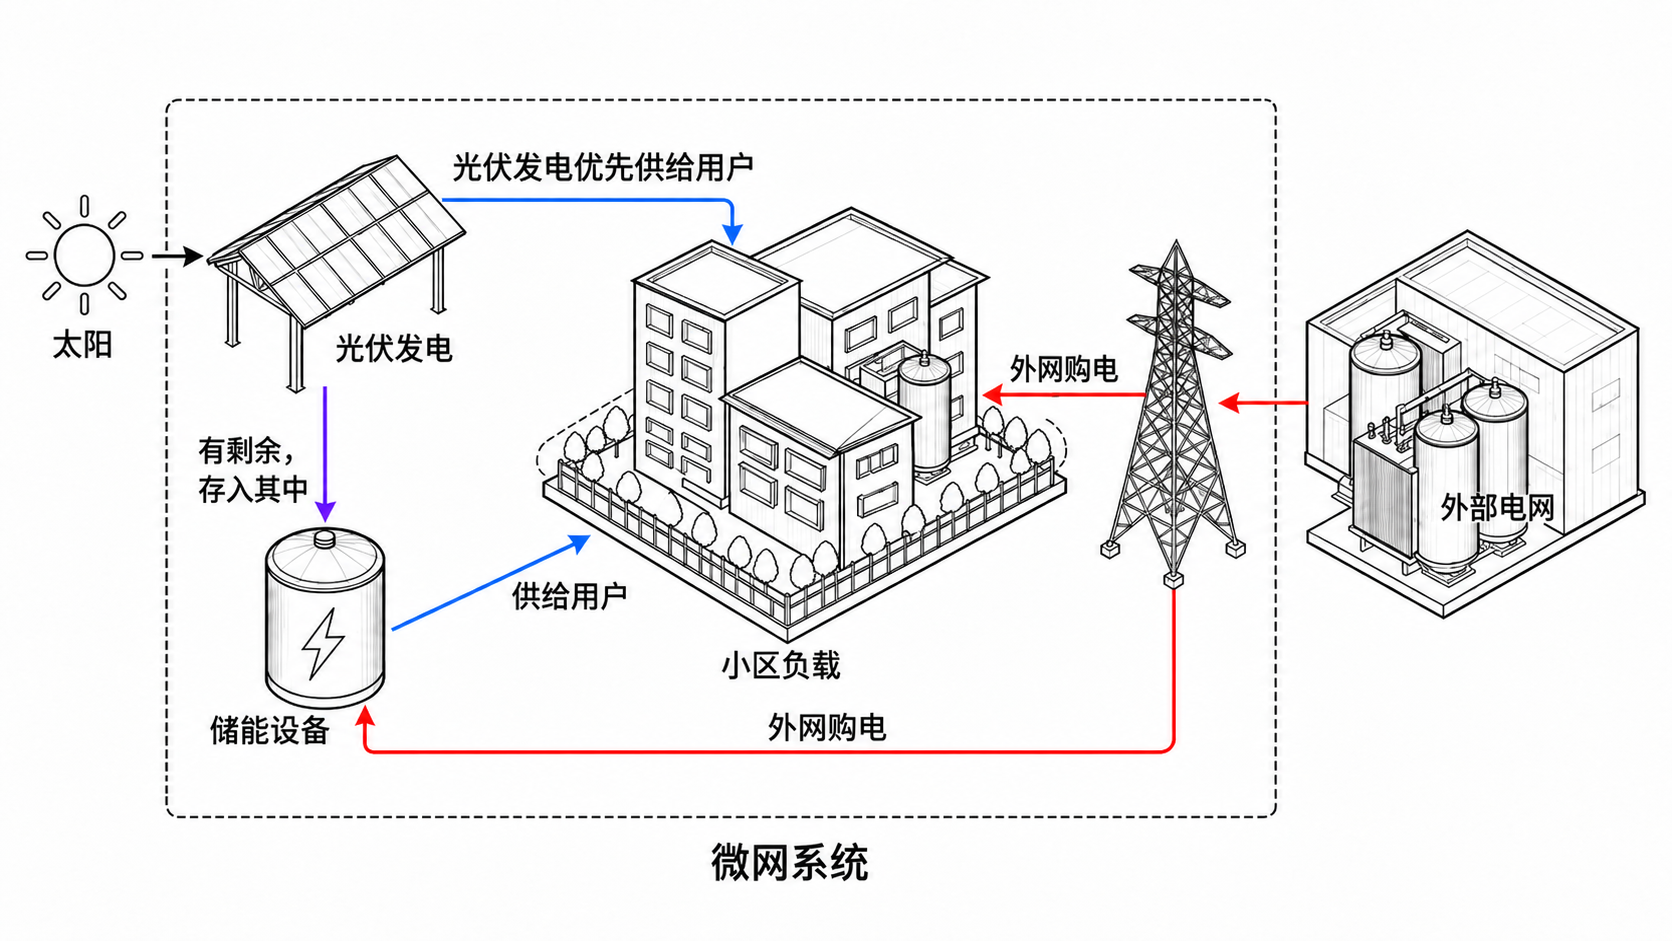
\includegraphics[width=0.78\textwidth]{fig/weiwang.png}
    \caption{微网系统流程图}
    \label{fig:weiwang}
\end{figure}

\subsection{问题提出}
\textbf{问题一：确定条件下的微网计划购电策略。}
已知一天内的负载、电价和光伏预测数据，制定当天的购电与储能充放电计划。
要求满足小区用电需求，并保证储能设备在 0:00 和 24:00 的电量相同，在此基础上尽量降低购电费用。

\textbf{问题二：实际供需变化下的每日购电。}
小区实际负载和光伏发电会随时间变化，因此每天都需要根据已有信息重新制定购电计划。
若实际供电不足，则需要按正常电价的 5 倍紧急购电，所以需要同时安排计划购电、储能使用和紧急购电，控制全年的总费用。

\textbf{问题三：利用更新的光伏预测调整购电计划。}
每天 0:00 先根据光伏预测制定计划，之后在 6:00、12:00 和 18:00 得到新的预测信息后，可以调整尚未执行的购电安排。
调整计划本身也会产生额外费用，因此需要比较“继续执行原计划”和“根据新预测进行调整”哪一种更划算，并判断是否有必要引入后续时刻的预测。

\textbf{问题四：波动电价下重新制定购电策略。}
进一步考虑外部电网电价随时间变化的情况，重新研究问题二和问题三中的购电与储能安排。
需要比较波动电价下的计划购电、储能使用、紧急购电和计划调整情况，并分析电价变化对微网购电策略和总费用的影响。